\documentclass[11pt]{beamer}
\usepackage[english]{babel}
\usepackage[T1]{fontenc}
\usepackage[utf8]{inputenc}
\usepackage{sourcesanspro}
\usepackage{sourcecodepro}
\usepackage{euler}
\usepackage[normalem]{ulem}
\usepackage{natbib}
\usepackage{apalike}
% \usepackage{bibentry}
% \usepackage{enumitem}
\usepackage[font={scriptsize},labelfont={scriptsize}]{caption}
\usepackage{lmodern,tgtermes,tabularx,ragged2e}
% \newcolumntype{Y}{>{\arraybackslash\RaggedRight}X}
% \newcolumntype{P}[1]{>{\arraybackslash\RaggedRight}p{#1}}
\usepackage{hhline}
\usepackage{booktabs}
\usepackage{array}
\newcolumntype{L}[1]{>{\raggedright\let\newline\\\arraybackslash\hspace{0pt}}m{#1}}
\newcolumntype{C}[1]{>{\centering\let\newline\\\arraybackslash\hspace{0pt}}m{#1}}
\newcolumntype{R}[1]{>{\raggedleft\let\newline\\\arraybackslash\hspace{0pt}}m{#1}}
\usepackage{makecell}
\usepackage{pdfpages}
% \usepackage[overlay,absolute]{textpos}
%   \setlength{\TPHorizModule}{1mm}
%   \setlength{\TPVertModule}{1mm}
\usepackage{graphicx}

% \nobibliography*
\setcitestyle{authoryear,comma,square,aysep={},yysep={}}
% \setbeameroption{hide notes}
% \setbeameroption{notes on second screen=right}
% \setbeameroption{use timer}
% \setbeameroption{use timer countdown=30}

\usetheme{inria}
%\usepackage{helvet}
\AtBeginSection[]{
  \begin{frame}[plain]
    \partpage
  \end{frame}
}
\newcommand{\inriaswitchcolors}[1]{%
\pgfaliasimage{figfootline}{figfootline-#1}% !!!
\pgfaliasimage{figbackground}{figbackground-#1}% !!!
\pgfaliasimage{figbackground}{figbackground-#1}% !!!
}
\setbeamertemplate{blocks}[rounded][shadow=true]
\setbeamercolor{block title}{fg=white,bg=inriaRed1}
\setbeamerfont{block title}{parent=frametitle,size=\small}
\setbeamerfont{section in toc}{parent=structure, size=\large}

% %remove the icon
% \setbeamertemplate{bibliography item}{}

% %remove line breaks
% \setbeamertemplate{bibliography entry title}{}
% \setbeamertemplate{bibliography entry location}{}
% \setbeamertemplate{bibliography entry note}{}

\usepackage{listings}
\usepackage{amsmath,amssymb}
% \usepackage{courier}

\usepackage{tikz}
\usepackage{tikz-cd}
\usetikzlibrary{decorations.pathreplacing,angles,quotes}
\usetikzlibrary{positioning}
\usetikzlibrary{shapes.geometric}
\usetikzlibrary{calc}
\usetikzlibrary{arrows,patterns}
\usetikzlibrary{intersections}
\usetikzlibrary{tikzmark,fit,shapes.geometric}

\definecolor{myviolet}{rgb}{0.6,0.0,0.65}
\definecolor{myblue}{rgb}{0.1,0.0,0.8}
\definecolor{mygreen}{rgb}{0.1,0.8,0.0}
\definecolor{myred}{rgb}{0.8,0.0,0.0}

\definecolor{dkblue}{rgb}{0,0.1,0.5}
\definecolor{lightblue}{rgb}{0,0.5,0.5}
\definecolor{dkgreen}{rgb}{0,0.4,0}
\definecolor{dk2green}{rgb}{0.4,0,0}
\definecolor{dkviolet}{rgb}{0.6,0,0.8}
\definecolor{shadethmcolor}{rgb}{0.9, 0.9,1}

\let\L=\lstinline
\def\lstlanguagefiles{defManSSR.tex}
\lstset{language=SSR}
\lstset{basicstyle=\footnotesize\ttfamily,breaklines=true}
\lstset{framextopmargin=50pt,frame=bottomline}
\lstset{moredelim=[is][\color{red}\bfseries\ttfamily\underbar]{|*}{*|}}
\lstset{moredelim=[is][\color{blue}\bfseries\ttfamily]{/*}{*/}}

\def\mathcomp{{\small\textsc{Mathematical Components}}}
\def\mydef#1{{\sl #1}}
\def\myem#1{{\bf\sl \color{red}{#1}}}
% \def\myem#1{\emph{#1}}

\newcommand{\cvg}[2]{#1 \rightarrow #2}
\newcommand{\abs}[1]{\left\lvert #1 \right\rvert}
\newcommand{\norm}[1]{\left\lVert #1 \right\rVert}
\newcommand{\scal}[2]{\left\langle #1, #2 \right\rangle}
\newcommand\IR{\ensuremath{\mathbb{R}}}
\newcommand\IC{\ensuremath{\mathbb{C}}}
\newcommand\nat{\ensuremath{\mathbb{N}}}
\newcommand\IN{\nat}

\renewcommand{\leq}{\leqslant}

\def\eps{\varepsilon}
\def\lip{LaSalle's invariance principle}
\def\o{\circ}
\def\coq{{\sc Coq}}
\def\ssr{{\sc SSReflect}}
\def\mathcomp{{\sc Mathematical Components}}
\def\coquelicot{{\sc Coquelicot}}
\def\isahol{{\sc Isabelle/HOL}}
\def\hol4{{\sc HOL4}}
\def\hollight{{\sc HOL Light}}
\def\lean{{\sc Lean}}
\def\pvs{{\sc PVS}}
\def\mizar{{\sc Mizar}}
\def\analysis{{\sc Mathematical Components Analysis}}
\def\plim{\Gamma^{+}}
\def\loc{\textrm{locally}}
\def\ball{\textrm{ball}}

\def\us{\char`\_}

\def\newterm#1{{\sl #1}} % to introduce new terms such as ``entourage'', etc.
\def\eg{\textit{e.g.}} % NB(rei): btw, the lncs authors' instructions uses the american convention (``e.g.,'' in roman)
\def\ie{\textit{i.e.}} % NB(rei): for uniformity (there was one with \em instead of \it)
\def\subset{\subseteq}
\def\supset{\supseteq}

% \makeatletter
% \renewenvironment{table}%
%   {\renewcommand\familydefault\sfdefault
%    \@float{table}}
%   {\end@float}
% \makeatother

\newcommand\doubleRule{\toprule\toprule}
\newcommand\doublerule{\toprule\specialrule{\heavyrulewidth}{\doublerulesep}{0.95em}}

\newcommand\coqPR[1]{\coq{} PR \href{https://github.com/coq/coq/issues/#1}{\##1}}
\newcommand\coqIssue[1]{\coq{} Issue \href{https://github.com/coq/coq/issues/#1}{\##1}}

\begin{document}

\title[Structure Hierarchies in Coq-ELPI]{{Generating Mathematical} {Structure Hierarchies} {using Coq-ELPI}}
\subtitle{FoMM, Pittsburgh, USA}

\author[\underline{Cohen}, Sakaguchi, Tassi]{
  \underline{Cyril Cohen \textit{(Inria)}}, Kazuhiko Sakaguchi, Enrico
Tassi}

% \institute[]{\inst{1} Inria, France, \inst{2} University of Tsukuba,
% Japan}

\date{January 6th, 2020}

\begin{frame}
\titlepage
\end{frame}

\begin{frame}[fragile]
  \frametitle{Structures in Mathematics}

  \begin{itemize}
  \item A \textbf{carrier} in Set / Type,
  \item A set of \textbf{constants} in the carrier, and \textbf{operations},
  \item Proofs of the \textbf{axioms} of the structure
  \end{itemize}

  \pause

\begin{lstlisting}
Record is_ring A := mk_ring {
    zero : A; add : A -> A -> A; opp : A -> A;
    one : A;  mul : A -> A -> A;
    addrA : associative add;
    addrC : commutative add;
    add0r : left_id zero add;
    addNr : left_inverse zero opp add;
    mulrA : associative mul;
    mul1r : left_id one mul;
    mulr1 : right_id one mul;
    mulrDl : left_distributive mul add;
    mulrDr : right_distributive mul add;
  }.
\end{lstlisting}

\end{frame}

\begin{frame}
  \frametitle{Structures in formalization}

  Purpose:
  \begin{itemize}
  \item factor theorems across instances, using the \textbf{theory} of
    each structure,
  \item \textbf{automatically find} which structures hold on which types.
  \end{itemize}

  \pause
  \vfill

  Requirements:
  \begin{itemize}
  \item declare a \textbf{new instance},
  \pause
  \item declare a \textbf{new structure}
    \begin{itemize}
    \item above, below or in the middle
    \item handle diamonds (e.g. monoid, group, commutative or not),
    \item by amending existing code, or not,
    \end{itemize}
  \pause
  \item \textbf{predictability} of inferred instance,
  \pause
  \item \textbf{robustness} of user code with regard to \textit{new declarations}.x
  \end{itemize}

\end{frame}

\begin{frame}[fragile]
  \frametitle{Structures relating to each other}

  Examples:

  \begin{itemize}
  \item Monoid $\leftarrow$ Group $\leftarrow$ Ring $\leftarrow$ Field
    $\leftarrow$ ...


  \item Euclidean Spaces $\rightarrow$ Normed Spaces $\rightarrow$
    Complete Space $\rightarrow$ Metric Spaces $\rightarrow$ Topological
    Spaces $\rightarrow$ ...

  \end{itemize}

  \pause
  \vfill{}
  
  \textbf{Going through arrows must be automated.}
  
  \pause
  \vfill{}

  Two kinds arrows:
  \begin{itemize}
  \item Extensions: add operations, axioms or combine structures
  \item Entailment/Induction/Deduction/Generalization.
  \end{itemize}

\end{frame}

\begin{frame}
  \frametitle{More examples}

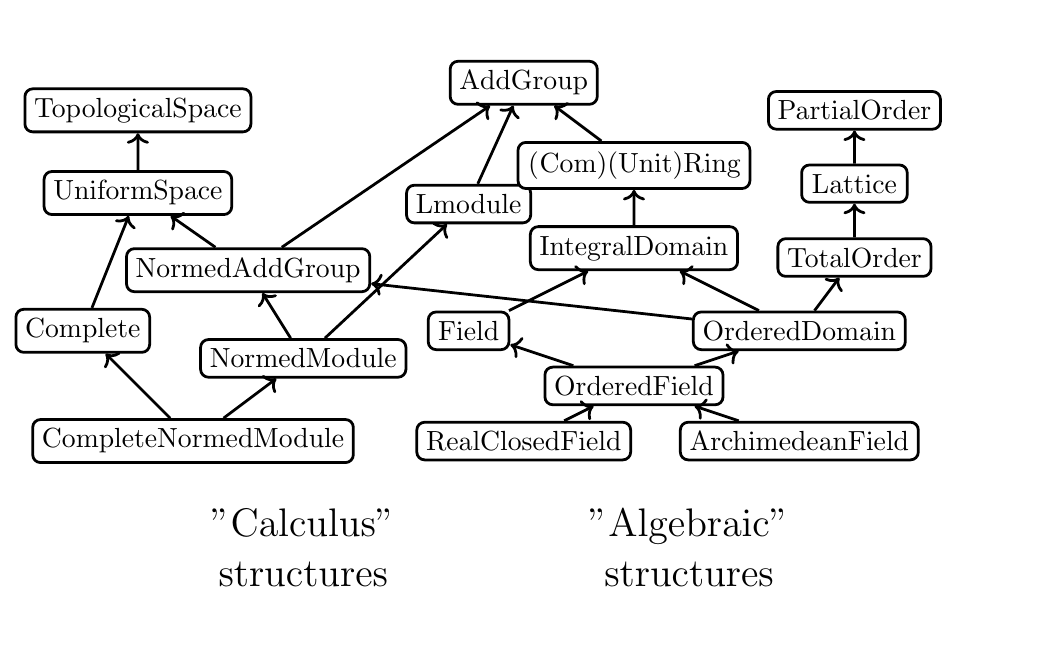
\begin{tikzpicture}[line width=1pt, structure/.style={draw, rounded corners=1mm, fill=white}, new/.style={preaction={fill, white}, pattern=crosshatch dots, pattern color=lightgray}, scale=0.7]
 \useasboundingbox (-6, -.5) rectangle (12, 10.5);
 % Replace `fill` with `pattern`s for the final version.
 %\draw[black!50, pattern=north east lines, pattern color=red!50, rounded corners=15mm] (-7.5, -.5) -- (-7.5, 7) -- (-4, 7) -- (2, 3) -- (2, -.5) -- cycle;
 %\draw[black!50, pattern=north west lines, pattern color=blue!50, rounded corners=15mm] (-8, -.5) -- (2, 4) -- (-4, 8) -- (0, 10) -- (10, 5) -- (10, -.5) -- cycle;
 %
 \node at (-1, 1) {\Large \begin{tabular}{c}''Calculus''\\structures\end{tabular}};
 \node at (6, 1) {\Large \begin{tabular}{c}''Algebraic''\\structures\end{tabular}};
 %
 \node[structure] (PartialOrder)          at (9,  9) {\L+PartialOrder+};
 \node[structure] (Lattice)         at (9,  7.67) {\L+Lattice+};
 \node[structure] (TotalOrder)           at (9,  6.33) {\L+TotalOrder+};
 %
 \node[structure] (AddGroup)             at (3,  9.5) {\L+AddGroup+};
 \node[structure] (Lmodule)              at (2, 7.3) {\L+Lmodule+};
 \node[structure] (Rings)                at (5,  8) {\L+(Com)(Unit)Ring+};
 \node[structure] (IntegralDomain)       at (5,  6.5) {\L+IntegralDomain+};
 \node[structure] (Field)                at (2,  5) {\L+Field+};
 \node[structure] (OrderedDomain)        at (8,  5) {\L+OrderedDomain+};
 \node[structure] (OrderedField)         at (5,  4) {\L+OrderedField+};
 \node[structure] (RealClosedField)      at (3,  3) {\L+RealClosedField+};
 \node[structure] (ArchimedeanField)     at (8,  3) {\L+ArchimedeanField+};
 %
 \node[structure] (TopologicalSpace)          at (-4, 9) {\L+TopologicalSpace+};
 \node[structure] (UniformSpace)              at (-4, 7.5) {\L+UniformSpace+};
 \node[structure] (Complete)             at (-5, 5) {\L+Complete+};
 \node[structure] (NormedAddGroup)       at (-2,  6.1) {\L+NormedAddGroup+};
 \node[structure] (NormedModule)         at (-1, 4.5) {\L+NormedModule+};
 \node[structure] (CompleteNormedModule) at (-3, 3) {\L+CompleteNormedModule+};
 %
 \draw[<-] (PartialOrder) to (Lattice);
 \draw[<-] (Lattice) to (TotalOrder);
 \draw[<-] (TopologicalSpace) to (UniformSpace);
 \draw[<-] (UniformSpace) to (Complete);
 \draw[<-] (UniformSpace) to (NormedAddGroup);
 \draw[<-] (Complete) to (CompleteNormedModule);
 \draw[<-] (Lmodule) to (NormedModule);
 \draw[<-] (NormedAddGroup) to (NormedModule);
 \draw[<-] (NormedModule) to (CompleteNormedModule);
 \draw[<-] (AddGroup) to (Lmodule);
 \draw[<-] (AddGroup) to (NormedAddGroup);
 \draw[<-] (AddGroup) to (Rings);
 \draw[<-] (Rings) to (IntegralDomain);
 \draw[<-] (IntegralDomain) to (OrderedDomain);
 \draw[<-] (NormedAddGroup) to (OrderedDomain);
 \draw[<-] (TotalOrder) to (OrderedDomain);
 \draw[<-] (IntegralDomain) to (Field);
 \draw[<-] (Field) to (OrderedField);
 \draw[<-] (OrderedDomain) to (OrderedField);
 \draw[<-] (OrderedField) to (RealClosedField);
 \draw[<-] (OrderedField) to (ArchimedeanField);

 % \draw[opacity=.5, black, fill=red!50, rounded corners=15mm] (-7.5, -.5) -- (-7.5, 7) -- (-4, 7) -- (2.5, 3) -- (2, -.5) -- cycle;
 % \draw[opacity=.5, black, fill=blue!50, rounded corners=15mm] (-8, -.5) -- (1.5, 4) -- (-4.3, 8) -- (0, 10) -- (10.5, 5.5) -- (10, -.5) -- cycle;
 \end{tikzpicture}

\end{frame}

\begin{frame}
  \frametitle{Structure extension}

  \begin{itemize}
  \item \textbf{Compositional}: no need to start from scratch every time.
    (E.g. the product of two groups is a group, the product of two
    rings is a ring),
  \pause\vfill
  \item \textbf{Noisy}: changes the internal definition of a structure.
    (E.g. Defining an commutative monoid from a monoid, we get already
    get one unnecessary axiom),
  \pause\vfill
  \item \textbf{Non-robust}: possible breakage of user code when new
    intermediate structures are added,
  \pause\vfill
  \item<4-> \textbf{Not all arrows!} \pause \alert{\textbf{Really?}}
  \end{itemize}

\end{frame}

\begin{frame}
  \frametitle{Structure entailment}

  \begin{itemize}
  \item \textbf{More flexible}: no need to cut structures into smaller
    bits.
  \item Cover the case of \textbf{all arrows}, including extensions.
    \pause\vfill
  \item Major breakage when arbitrary entailment is automatic;

    e.g. given two normed spaces, and making their Cartesian product, in
    order to obtain the resulting topology, one can either:
    \begin{itemize}
    \item first consider the normed space product, then derive the
      corresponding topological space, or
    \item first derive the topological spaces and then consider the
      topological space product.
    \end{itemize}
  \end{itemize}

\end{frame}

\begin{frame}
  \frametitle{Our Design}

  The best of two the worlds:
  \begin{itemize}
  \item \textbf{Extension}, through \emph{mixins} for \textbf{internal declaration} and
    \textbf{automatic inference}

  \item \textbf{Entailment}, through \emph{factory} for any other use.

    Factories require mixins and can produces others.
    (e.g. a full axiomatic can provide all the pieces)
  \end{itemize}

  \pause  \vfill

  We generate and generalize the design from \textit{Packaging
    Mathematical Structures} (Garillot \textit{et al.}) and
  \textit{Canonical Structures for the working Coq user} (Mahboubi and
  Tassi).

  \pause  \vfill

  We follow a fully bundled approach, where carriers are packaged
  together with their axiomatic.
  
\end{frame}


\begin{frame}[fragile]
  \frametitle{Hiearchy builder at work}
  
  Five commands:
  \begin{itemize}
  \item \L{declare_mixin FactoryModuleName TypeName Factories.}
  \item \L{declare_factory FactoryModuleName TypeName Factories.}
  \item \L{end Functions.}
  \item \L{structure ModuleName Factories.}
  \item \L{instance Carrier Factories.}
  \end{itemize}
  \vfill
  \begin{center}
    Demo

    \url{https://github.com/math-comp/hierarchy-builder}
  \end{center}
  
\end{frame}

\begin{frame}
  \frametitle{Conclusion}
  
  \begin{itemize}
  \item High-level commands to declare structures and instances, \\
    easy to use.
    \vfill
  \item Predictable outcome of inference,
    \vfill
  \item Takes into account the evolution of knowledge
    \begin{itemize}
    \item which is formalized, and
    \item which the user has.
    \end{itemize}
    The two knowledge do not need to be correlated.
    \vfill
  \item Robustness with regard to new declaration \emph{and even changes of
    internal implementation}.
  \end{itemize}
  
  \vfill\pause
  Also, \textsc{Coq-ELPI} turned out to be a very comfortable
  meta-programming language for this.

\end{frame}

\begin{frame}
  \frametitle{Future work on Hierarchy Builder}
  \begin{itemize}
  \item Adding support for parameters.
    \vfill
  \item Generating hierarchies of morphisms from structures.
    \vfill
  \item Generating hierarchies of subobjects from structures.
    \vfill
  \item Supporting multiple instances on the same carrier.
    \vfill
  \item Replacing all uses in math-comp and extensions.
    \vfill
  \item Get better error messages.
  \end{itemize}
\end{frame}

\end{document}
